
\documentclass[12pt]{article}


\usepackage[utf8]{inputenc}
\usepackage[bulgarian]{babel}
\usepackage{graphicx}
\graphicspath{ {./images/} }
\usepackage{sidecap}  %required for side captions
\usepackage{amssymb}
\usepackage{amsmath}
\usepackage{hyperref}
\usepackage{commath}  
\usepackage[top=1.3in, bottom=1.5in, left=1.3in, right=1.3in]{geometry}


\begin{document}
	\begin{center}
        \LARGE{\textbf{Тема: SNS симулатор}}
        
        \bigskip
        \Large{Предмет: Приложно-програмни интерфейси за работа с облачни архитектури с Амазон Уеб Услуги (AWS)}
        
        \medskip
        \Large{Изготвил: Борислава Анатолиева Багалийска, фн: 81665, имейл: bbagaliyska@gmail.com}
        
        \medskip
        \Large{Лектор: доц. Милен Петров, година: 2019/2020}
        
        \bigskip
	\end{center}
    
    
  %  \newpage
    \tableofcontents
    \bigskip
    \bigskip
    \newpage
  
\section{Условие} 

\noindent Serverless симулация на услугата SNS на AWS.

\medskip


\noindent SNS е услуга за изпращане на известия към различни видове получатели. 
Във варианта, в който е реализиран в проекта, възможни получатели на съобщения
могат да бъдат HTTP URL-и, AWS Lambda функции, AWS SQS опашки за съобщения и
имейл клиенти.

\section{Въведение}

Тъй като в основата на AWS услугите е те да са скалируеми и с висока наличност,
избрах да реализирам всички функционалности от условието в AWS пространството, 
възползвайки се от стабилността и свойствата на различните услуги, които то предлага.
Избрах имплементацията да е serverless, защото нямах опит с подобни приложения досега 
и мисля, че предлага по-голяма гъвкавост за подобрение и разширение на решението, както
и по-ефикасно използване на хардуерните ресурси.

\noindent Популярна опция за вдигане на serverless приложение, използвайки AWS e използване на
комбинация от AWS Lambda и DynamoDB, което е и начина, по който е организирана и инфраструктурата
на проекта. AWS услугите, използвани в решението са:

\begin{itemize}
    \item Lambda
    
    \item DynamoDB
    
    \item SQS
    
    \item SES
    
    \item IAM
\end{itemize}

\section{Теория}
\noindent Ще опиша различните лимитации на двете основни използвани услуги и как е добре да се адресират.

\medskip

\noindent Използвайки лимитите по подразбиране, \textbf{AWS Lambda} поддържа 1000 конкурентни изпълниния,
75GB данни, от които за едно асинхронно извикване са позволени 256 KB, а за синхронно - 6 MB.
Текущото решение не се опитва да оптимизира тези стойности, но със сравнително малко промени би могло
да го прави. Идеята на всяка функция е да има сравнително лека и бърза задача и при нужда да се обръща
към други Lambda функции, за да реализират различни подзадачи. Подобно нещо се случва при основната
Lambda, приемаща заявка за изпращане на съобщение, която делегира към Lambda функции, обработващи само 
един вид съобщения. Това, което не е взето предвид е големината на входните данни - хубаво е ако надвишават
горепосочените лимити, да се разбиват на по-малки блокове и да се дават за паралелна обработка от няколко
инстанции на Lambda функции.

\noindent \textbf{DynamoDB} предлага по 40,000 единици заявки за четене и 40,000 единици заявки за писане
на таблица. Приложението използва една таблица, така че това са и лимитите на приложението. Единицата в
случаи на консистентно четене представлява едно четене в секунда на данни до 4KB; съответно едно писане
в секунда на данни до 1KB. За писане това е предостатъчно, тъй като начина на използване на приложението
най-вероятно няма да води до толкова чести записи - записът представлява добавяне на тема или абонат към тема.
Към момента приложението е направено така, че да се инсталира локално в инсфраструктурата на всеки ползващ го
потребител, така че за един потребител при нормална употреба тези стойности са недостижими.
Вътрешно при изпращане на съобщение се четат всички абонати към съответната тема от базата и ако те са
много на брой е възможно да трябва да се чете на части от няколко инстанции на ламбди, но това не е
реализирано. Адресирах възможността за паралелни заявки, като структурирах данните по определен начин в
таблицата в различни атрибути от тип StringSet, защото по този начин може добавянето и махането на 
абонат да стане в една заявка вместо с две (четене и после промяна) и така процеса е атомарен, стига
вътрешно AWS да са реализирали атомарно заявката.

%\newpage

\section{Използвани технологии}
Първоначално бях замислила да се използва Java 11, но реших да експериментирам с Python 3.8, с който
не бях работила досега, но изглеждаше като удобен избор за целта.
\begin{itemize}
    \item \textbf{Python} - version 3.8.
    
    \item \textbf{boto3} - version 1.13.9.
\end{itemize}

%\newpage

\section{Инсталация и настройки}
\noindent\textbf{Стъпка 1.} Вдигане на нужната инсфраструктура, зададена във файла configurations.md

\medskip

\noindent\textbf{Стъпка 2.} Сваляне на клиентската библиотека на Python 3

\section{Кратко ръководство за потребителя}

\noindent Графики, които описват движението на контрола при заявка от потребителя:

\noindent Създаване на тема

\begin{figure}[h!]
\centering
    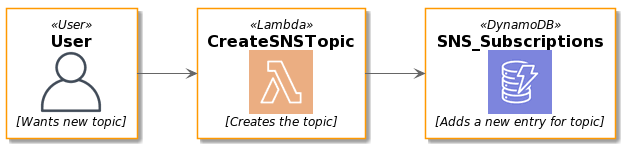
\includegraphics[scale=0.4]{topic_creation_flow.png}
    \caption{Създаване на тема}
\end{figure}

\noindent Изтриване на тема

\begin{figure}[h!]
  \centering
      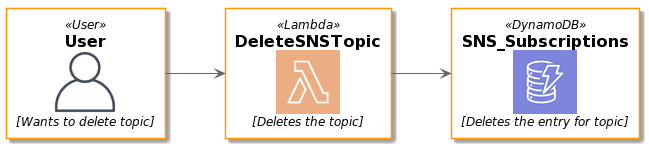
\includegraphics[scale=0.4]{topic_deletion_flow.png}
      \caption{Изтриване на тема}
\end{figure}

\noindent Добавяне на абонамент

\begin{figure}[h!]
  \centering
      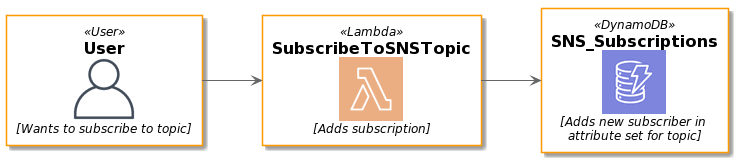
\includegraphics[scale=0.4]{subscription_creation_flow.png}
      \caption{Добавяне на абонамент}
\end{figure}

\noindent Премахване на абонамент

\begin{figure}[h!]
  \centering
      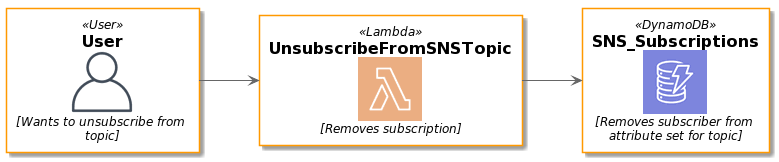
\includegraphics[scale=0.4]{unsubscription_flow.png}
      \caption{Премахване на абонамент}
\end{figure}

\noindent Изпращане на съобщение

\begin{figure}[h!]
  \centering
      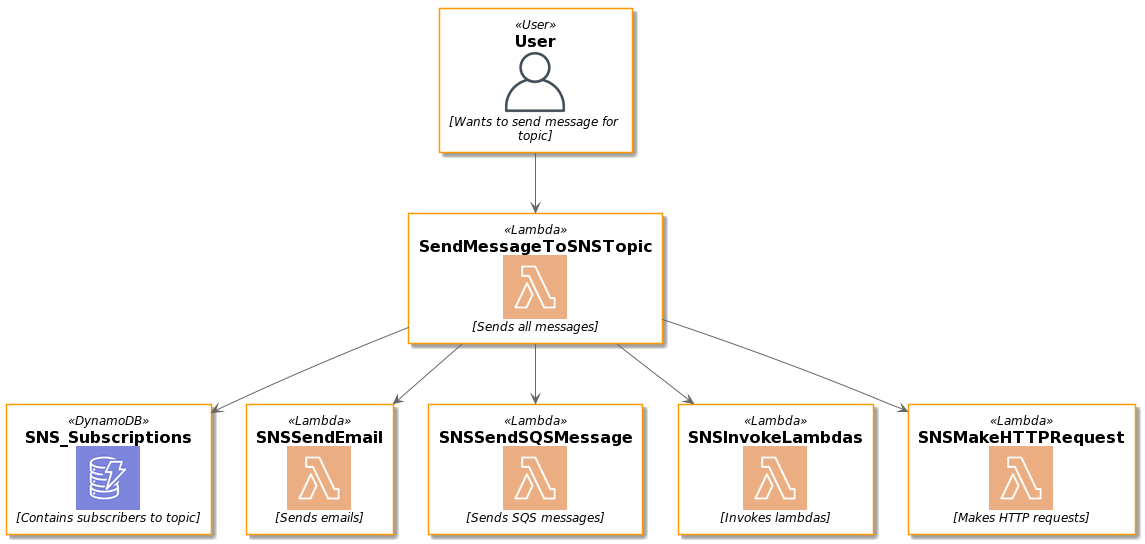
\includegraphics[scale=0.4]{message_sending_flow.png}
      \caption{Изпращане на съобщение}
\end{figure}

\section {Примерни данни за SNS\_Subscription таблицата}

\begin{table}
\caption{SNS\_Subscriptions DynamoDB table - Emails}
\center
\begin{tabular}{ |c|c| }
 \hline
 Topic & email\_subscribers \\ \hline

 news & \{"email1\@gmail.com" \, "email2\@gmail.com"\} \\
 software-updates & \{'email3\@gmail.com'\} \\ 
 \hline
\end{tabular}
\end{table}

\begin{table}
\caption{SNS\_Subscriptions DynamoDB table - SQS}
\center
\begin{tabular}{ |c|c| }
 \hline
 Topic & sqs\_subscribers \\ \hline

 news & \{"https://sqs.region-name.amazonaws.com/account-id/queue-id"\} \\
 software-updates & \{\} \\ 
 \hline
\end{tabular}
\end{table}

\begin{table}
\caption{SNS\_Subscriptions DynamoDB table - Lambda}
\center
\begin{tabular}{ |c|c| }
 \hline
 Topic & lambda\_subscribers \\ \hline

 news & \{\} \\
 software-updates & \{"arn:aws:lambda:region-name:account-id:function:lambda-id"\} \\ 
 \hline
\end{tabular}
\end{table}

\begin{table}
\caption{SNS\_Subscriptions DynamoDB table - HTTP}
\center
\begin{tabular}{ |c|c| }
 \hline
 Topic & http\_subscribers \\ \hline

 news & \{\} \\
 software-updates & \{"https://www.google.com/"\} \\  
 \hline
\end{tabular}
\end{table}

 
\section{Описание на програмния код}

\subsection{Функции за работа с DynamoDB}
\begin{itemize}
  \item CreateSNSTopic
  \item DeleteSNSTopic
  \item SubscribeToSNSTopic
  \item UnsubscribeFromSNSTopic
  \item SendMessageToSNSTopic
\end{itemize}

\subsection{Функции за работа с други AWS Lambdas}
\begin{itemize}
  \item SNSInvokeLambdas
  \item SendMessageToSNSTopic
\end{itemize}

\subsection{Функции за работа с AWS SQS}
\begin{itemize}
  \item SNSSendSQSMessage
\end{itemize}

\subsection{Функции за работа с AWS SES}
\begin{itemize}
  \item SNSSendEmail
\end{itemize}

\medskip

Базата данни е реализирана като има ключ (partition key) - темата.
За всяка тема (topic) се пазят по един атрибут за всеки тип абонамент -
имейл, HTTP, SQS, Lambda.
Тези атрибути представляват StringSets от идентификатори на абонираните ресурси.
За тип имейл - множество от имейли, към които да се пращат електронни съобщения -
в случаи на потребители в SandBox тези имейли трябва да бъдат верифицирани в SES
За тип HTTP - множество от URL-и, към които да се пращат POST заявка 
За тип SQS - множество от URL идентификатори на SQS опашки, за които съответния
потребител трябва да има достъп да изпраща съобщение
За тип Lambda - множество от ARN идентификатори (може и имена) на Lambda функции, 
които съотвения потребител трябва да има право да изпълнява
В тази база се записват новите теми и абонати и от нея се четат, когато трябва да се
изпрати съобщение.


\section{Приноси на студента, ограничения и възможности за бъдещо развитие}

\subsection{Приноси на студента}
Реализирана е основната функционалност на SNS, използвайки редица AWS услуги,
severless approach и избор на програмен език и инструменти, които позволяват 
изчистена и ясна имплементация, отворена към разширение на функционалностите и 
реализиране на основни нефункционални изисквания, на които се базира AWS: 
high availability, scalability, durability, security.

\medskip

\subsection{Ограничения} 
Реализацията към момента се ограничава от това, че инфраструктурата се инсталира в
локалното AWS пространство на всеки използващ го потребител, вместо да се обръща към
endpoints. Това решение е взето главно заради това, че услугите не са безплатни и студентският
акаунт е по-скоро тестови цели и лимитиран. Лесно може да се мине и на централно решение без да 
се модифицира текущия код. Други ограничения са свързани с ограниченията в капацитета на ламбдите,
които могат да се адресират с вкарване на паралелизъм, четене от базата на по-малки порции и 
пускане на повече от една ламбда за една задача, но не успях да реализирам тези неща от времеви
ограничения.

\subsection{Възможности за бъдещо развитие}
\begin{itemize}
  \item Поддържане на други типове абонаменти - като пращане на SMS или push notifications
  \item Пазене на мета информация за всеки тип тема или потребител, които да могат да се конфигурират при създаване
  \item Вкарване на многонишково програмиране и on-demand викане на нужния брой ламбди за обработване на по-големи заявки
  \item Интегриране с Dead Letter Queue и/или CloudWatch за автоматизирано проследяване на грешките при изпращането на съобщения
  \item Създаване на CloudFormation script за бърза инсталация на нужната инфраструктура
  \item Създаване на Command Line Interface tool за работа с услугата
\end{itemize}

\section{Какво научих}
Добих полезен опит с езика Python, който беше нов за мен.
След доста прекарано време в четене на AWS документация и експерименти с услугите,
вече имам основна обща представа за това как се работи със средствата на AWS, за Какво
бих могла да ги ползвам и колко лесно и интуитивно е да се интегрират в едно приложение.
Осъзнавам, че предимствата, които предлагат от страна на капацитет, сигурност и динамична 
скалируемост са много трудни (ако не и невъзможни) за постигане от един обикновен екип, работещ
по някакъв проект и нуждаещ се от тези свойства като основа, върху която да пишат и специфичната
бизнес логика. Затова ако приложението, върху което работя, се нуждае от такива големи ресурси и
възможности, не бих се поколебала да се възползвам от AWS.

\section{Списък с фигури и таблици}

\listoftables

\listoffigures

\section{Използвани източници}

\noindent\href{https://boto3.amazonaws.com/v1/documentation/api/latest/index.html}{[1] Python 3 AWS SDK Documentation}
\noindent\href{https://docs.aws.amazon.com/}{[2] Official AWS Documentation}

\medskip


\bigskip


\end{document}